\chapter{Methodology}
\label{ch:methodology}

In this chapter it will be explained how the clustering experiments were conducted. The first part of the chapter is dedicated to define some concepts related to the On Target product: the OT itself, its benchmark project and how the environment for the experiments was set. The second part is about the procedures: to analyse the data, to cluster the data and to run the OT with the clustering results.

\section{About the Product}

Before getting to the clustering and experiment procedures, it is important to define some concepts about the OT product. A high level explanation of the OT, how its benchmark was build and the setup of the environment of the experiments will be described in this first part of the chapter.

\subsection{On Target}

The On Target is one of the Neoway's products of the vertical of Sales and Marketing. It is a content-based recommender system that searches for leads based on the customers' profile of the user. The OT receives as input:
\begin{itemize}
    \item the \textbf{Portfolio}, which is the list of companies that are customers of the OT user. It can range from a few dozens to dozens of thousands companies;
    \item the \textbf{Market}, which is the list of companies where the OT will search for the leads. It can range from dozens to tens of millions companies; and
    \item the \textbf{Features}, which is a data set with the characteristics of the companies.
\end{itemize}
And it outputs the sorted \underline{Market} based on a score called \textbf{Similarity}. Figure \ref{fig:ot-blocks} illustrates a block diagram of the OT.

\begin{figure}[h]
   \centering
   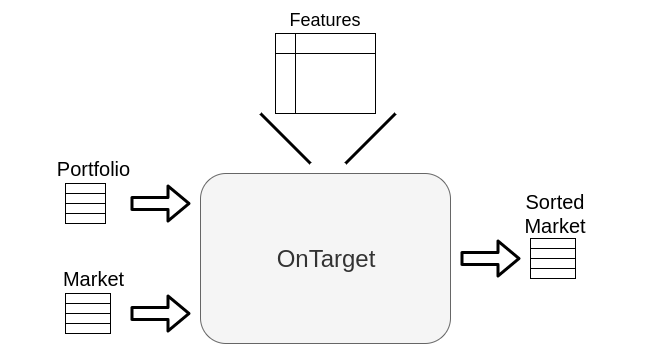
\includegraphics[width=\linewidth]{fig/ch3-ot-blocks.png}
   \caption{Block Diagram of the On Target. Source: Author}
   \label{fig:ot-blocks}
\end{figure}

\subsection{Benchmark}

As mentioned on the chapter \ref{ch:introduction}, the recommender system was update and one of the ways to assure that the modifications had a positive impact on the algorithm was to develop a benchmark. It is a project that compares different versions of the OT, by running these versions on almost thirty different business scenarios. They can be: one retail customer with a huge portfolio and huge market size; or a bank with a small portfolio and medium market size; or even a service provider with small portfolio and small market size. A run of the OT for one of this scenarios is called a \textbf{Study}. An \textbf{Experiment} is the run of all of these scenarios for new versions of the OT comparing to the current one that it is running on production. Every modification on the algorithm generates a new experiment. For instance, if the number of features is increased, an experiment (or more) is generated. If a parameter of the algorithm is changed, a new experiment is generated.

The Benchmark does some minor modification on the OT pipeline. It removes a random sample of companies from the portfolio (it can be 10\%, 30\% or 50\%) and it places them on the market. The idea is to use this sample as holdout set \cite{kohavi2001}, which is a separated part of the data used for test. The OT doesn't "know" that these companies are from the portfolio, therefore it is expected that they have a high score (similarity) on the output. Figure \ref{fig:ot-benchmark-blocks} shows these modifications on the OT.

\begin{figure}[h]
   \centering
   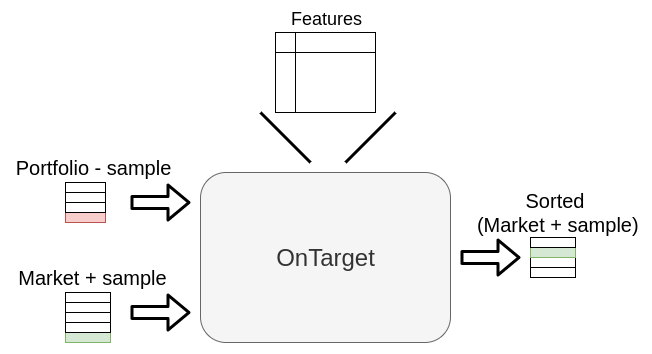
\includegraphics[width=\linewidth]{fig/ch3-ot-benchmark-blocks.png}
   \caption{Modifications on the OT done by the Benchmark. Source: Author}
   \label{fig:ot-benchmark-blocks}
\end{figure}

These changes on the pipeline are to generate the metrics to evaluate the experiments in two ways. The first one, is the performance with the \textbf{lift}, usually through a plot. The second one is consistency, with the \textbf{similarity distribution} plot. On the former, the holdout set is used to calculate the probabilities after the sorting of the OT - similar to the red balls analogy discussed on \ref{ch:evaluation}. The latter, plots the distribution of the scores assigned to the market and to the holdout set. As seen on the Introduction chapter of this work, Figure \ref{fig:simi-dist-expected-real} shows an example of this plot, where the orange are the holdout set and the blue curve is the market.

%\subsection{Experimental Environment}
%In order to not disrupt the production and development environment of the OT, it was set a separated environment to develop the experiments. A remote cluster with all the OT and benchmark code with a jupyter notebook as set.
% Not sure if need to talk about this

\section{Clustering}


\section{Experiments}

\subsection{One run by Clusters}

\subsection{Cluster as features}
